\chapter{Implementation}

% \section{Overview}

In this section we outline the general structure and design choices that went into the implementation of this process. 
While we wont go into the minutiae of the source code, it can be found at the GitHub repository...\question{GitHub link?}
The project is primarily implemented using three different frameworks: PyTorch, PyTorch Lightning and Hydra.
PyTorch provides the base deep learning methods, while PyTorch Lightning also provides a bunch of additional features, such as handling of different computational devices such as GPU, handling the different train, validation and test data splits, an extensive callback API and more.
Importantly, PyTorch Lightning also provides encapsulation of the inference process through the use of LightningModules.
A goal for the implementation has been to separate the modelling, the data and the inference methods as much as possible.
This makes it possible to effectively compare different methods of inference across different models and data.
The overall architecture can be seen in \cref{fig:sw-arch}.
\begin{figure}[htbp]
    \centering
    % spellchecker: disable

\begin{tikzpicture}[
    class/.style={rounded corners=0.3cm,minimum height=1cm,fill=blue!50,draw=black},
    back group/.style={rounded corners, draw=black, 
                     dashed, inner xsep=0.2cm, inner ysep=0.3cm, 
                     anchor=west},
    node distance = 1cm, 
    auto
    ]
    \node[class,fill=brightgreen!50] (sgd-module) at (2, 4.75) {SGDInference};
    \node[class,right=0.2cm of sgd-module.east,fill=brightgreen!50] (vi-module) {VariationalInference};
    \node[class,right=0.2cm of vi-module.east,fill=brightgreen!50] (mcmc-module) {MCMCInference};
    \node[class,above=1.2cm of mcmc-module] (sampler) {Sampler};
    \begin{scope}[on background layer]
        \node (inf-modules) [back group] [fit=(sgd-module)(vi-module)(mcmc-module),label={below right:InferenceModule}]{};
    \end{scope}
    \node[class, left=of inf-modules] (data-module) {DataModule};
    \node[class, above=1cm of data-module] (dataset) {Dataset};
    \node[class, align=center, above=2cm of inf-modules] (conv) {Bayesian-\\ConversionConfig};
    \node[class,left=1cm of conv] (model) {Model};
    \path (data-module) -- (mcmc-module) node[midway] (center) {};
    \node[class, below=2.5cm of center, fill=grey] (trainer) {pl.Trainer};
    % \node[class] (8) at (3.5, 7) {Priors};
    \draw [->] (sampler) -- (mcmc-module);
    \draw [->] (model) edge (mcmc-module);
    \draw [->] (model) edge (vi-module);
    \draw [->] (model) edge (sgd-module);
    \draw [->] (conv) edge (mcmc-module);
    \draw [->] (conv) edge (vi-module);
    \draw [->] (conv) edge[dashed] (sgd-module);
    \draw [->] (dataset) -- (data-module);
    \draw [->] (data-module) edge[out=-90, in=90] (trainer);
    \draw [->] (inf-modules) edge[out=-90, in=90] (trainer);
\end{tikzpicture}

    \caption{Overall architecture of inference implementation. }
    \label{fig:sw-arch}
\end{figure}

\section{Models}
The models used in this project are defined in the \texttt{src/models} directory.
These are implemented as PyTorch modules with some additional methods that are used by the other components. 
At a high level, they define some amount of trainable parameters $\theta$, as well as a mapping from input $x$ to output $y=f_\theta(x)$. 
They also define an observation model through $p(y|x, \theta)$ using the distribution objects provided by PyTorch.
These model does not provide any probabilistic assumptions about model parameters.
They are instead applied dynamically to each model according some configuration, which allows for 
In practice, for the bayesian methods, each Pytorch module with learnable parameters is changed for a Bayesian copy that also includes information about the parameter priors.

\section{Data}
Data is represented by PyTorch datasets.
The dataset abstraction is implemented using two methods, one for getting the total size of the dataset $N$, and another for getting extracting the $i$th observation.
For use with PyTorch Lightning these dataset are then wrapped in a \texttt{pl.LightningDatamodule} object, which defines how the data should be used during training, specifying data splits, batch sizes etc.
For this project, a general \texttt{pl.LightningDatamodule} implementation, \texttt{DataModule} is used in order to reduce code duplication and better be able to ensure consistency between experiments. 

\section{Inference Modules}
The inference modules defines the different means of inference and are initialized using a model object alongside any inference hyper-parameters.
The modules are implemented as \texttt{pl.LightningModule}s, and are therefore meant to be used with the \texttt{pl.Trainer} object alongside a \texttt{pl.Datamodule} for model fitting. 
There are three different inference methods implemented: regular stochastic gradient descent, variational inference and inference using Markov chain Monte Carlo inference.

In order to implement probabilistic methods, we have to supply the inference methods with additional information in form prior probabilities of the parameters. 
These are specified using a user specified Bayesian conversion configuration.
We then substitute each module with trainable parameters with a corresponding Bayesian module, which also defines parameter priors, as well a method for calculating the prior log probability.
The dynamical approach is chosen since it makes specifying the models simpler, allows for adjusting the priors dynamically and differently based on the methods in question, and also allows for training of models specified elsewhere like pre-trained models. 
For comparison with the probabilistic methods, the SGD inference optionally allows for using MAP estimation also using this framework.

At the core, the PyTorch Lightning framework is centered around the implementation of a \texttt{training\_step()} method.
This function gets as argument a batch of training data and is supposed to return the corresponding loss.
The Lightning framework then deals backwards pass, enabling and disabling gradients, pre-fetching data, moving values across different devices and so on.
For SGD inference it is therefore as simple as calculating the loss and passing it along.
For the two other methods the implementation is a bit more involved.

\subsection{Variational Inference}
\begin{figure}[htbp]
    \centering
    \begin{subfigure}[c]{0.48\linewidth}
        \centering
        % spellchecker: disable


\usetikzlibrary{shapes.multipart}
\begin{tikzpicture}[
    class/.style={rounded corners=0.3cm,minimum height=1cm,fill=blue!50,draw=black},
    other/.style={circle,draw=black},
    node distance = 1cm, 
    myrect/.style={
        draw,
        rectangle split,
        rectangle split parts=#1,
        rectangle split part align=left
        },    
    back group/.style={rounded corners, draw=black, 
                    dashed, inner xsep=0.2cm, inner ysep=0.2cm, 
                    anchor=west},
    auto
    ]
    \node[
        draw, 
        rectangle, 
        rectangle split, 
        rectangle split parts=7,
        rectangle split horizontal, 
        rectangle split part fill={
            grey,
            grey,
            brightgreen,
            white,
            white,
            white,
            white
            },
        minimum height=1cm,
        inner sep=2,
        rounded corners=0.1cm
        ] (samples) {
            \nodepart{one}
            \nodepart{two}
            \nodepart{three} \texttt{i}
            \nodepart{four}
            \nodepart{five}
            \nodepart{six}
            \nodepart{seven}
        };
    \node[class,fill=blue!50, below=1.5cm of samples] (bayesian-module) {BayesianModule};
    % \begin{scope}[on background layer]
        % \end{scope}
    \draw [->] (samples.three south) -- (bayesian-module.north -| samples.three south);
    \draw[decorate,decoration={brace, amplitude=10pt, raise=2pt}]
    (samples.one north) to node[black,midway,above=10pt] (samples-label) {$n$ samples} (samples.seven north);%
    \node (inf-modules) [back group] [fit=(bayesian-module)(samples)(samples-label),label={above:VariationalModule}]{};
    \node [other,left=of bayesian-module] (input) {$x$};
    \node [other,right=of bayesian-module] (output) {$x^\prime$};
    \draw [->,thick] (input) -- (bayesian-module);
    \draw [->,thick] (bayesian-module) -- (output);
    \draw [->,thick](bayesian-module.east) to[out=0,in=330, edge node={node [sloped,above] {\tiny \texttt{i++}}}] (samples.south east);
    \end{tikzpicture}

    \end{subfigure}
    \hfill{}
    \begin{subfigure}[c]{0.48\linewidth}
        % spellchecker: disable


\usetikzlibrary{shapes.multipart}
\begin{tikzpicture}
    \node[class] (model) at (0, 0) {Model};
    \node[fill=grey!50,other,below=1cm of model.south] (obs) {$\tilde{\D}$};
    \node[other,right=1.5cm of model] (loss) {$\bar{\mathcal{L}}$};

    \def\tsh{0.7cm}
    \node[minimum width=0.5cm, above=\tsh of model,anchor=center,label={above:{\tiny\texttt{training\_step()}}}] (training-step) {};

    \node[pnt] (start) at (training-step.west) {};
    \node[pnt] (end) at (training-step.east) {};
    \fill[black] (start) circle (2pt);
    \fill[black] (end) circle (2pt);
    \def\radius{1cm}

    \draw[ 
        flow,
        thick,
        postaction={decorate},
        decoration={
            markings,
            mark=at position 0.125 with {\arrow {latex}},
            mark=at position 0.375 with {\arrow {latex}},
            mark=at position 0.625 with {\arrow {latex}},
            mark=at position 0.875 with {\arrow {latex}}
        }
    ]
    (start)
    arc (90:180:\radius) node (tmp1) {}
    --
    ($(tmp1)!2.0!(tmp1 |- model)$) node[midway,anchor=center,label={left:\small{sample $n$}}] (sample-n) {}
    arc (180:270:\radius) node (tmp2) {}
    -- (tmp2 -| end) node[midway,anchor=center] (get-obs) {}
    arc (270:360:\radius) node (tmp3) {}
    -- ($(tmp3)!2.0!(tmp3 |- model)$) node[midway,anchor=center] (get-loss) {}
    arc (0:90:\radius) {}
    ;
    \def\radcirc{0.7}
    \draw[flow,thick,postaction={decorate},
        decoration={markings,
        mark=at position 0.27 with {\arrow {latex}},
        mark=at position 0.52 with {\arrow {latex}},
        mark=at position 0.77 with {\arrow {latex}}
    }]
    (get-obs.center) 
    arc (90:0:\radcirc) 
    arc (360:90:\radcirc) node[pos=0.333,anchor=north] (label) {\small repeat $n$ times}
    ;
    
    \fill[black] (sample-n) circle (2pt);
    \fill[black] (get-obs) circle (2pt);
    \fill[black] (get-loss) circle (2pt);
    
    \draw [depends] (obs) edge (model);
    \draw [depends] (model) edge (loss);
    \draw [depends] (sample-n.center) -- (model);
    


    \end{tikzpicture}

    \end{subfigure}
    \caption{Joint distribution of samples for $a_1$ and $a_3$ for the polynomial regression example for HMC and SGHMC for different batch sizes, with the actual posterior density also shown.}
    \label{fig:vi-arch}
\end{figure}

\subsection{MCMC Inference}
The Markov chain Monte Carlo implementation differs a bit compared to the two other implemented methods, in that we need to do more with the gradient, than just perform an optimization step. 
It is probably possible to use PyTorch Lightning's \texttt{on\_after\_backward()} hook to implement the HMC methods in PyTorch Lightning, however with this implementation we instead opt to implement the sampling algorithms more explicitly.
This allows for a simpler implementation of the samplers, that can be used also for eg. sampling from a density function directly.
The different samplers are therefore implemented as  subclasses of the \texttt{Sampler} class, that each defines a \texttt{next\_sample()} method independently.
After initializing each sampler, they are set up by registering to them an object defining what distribution should be sampled from. 
This object, dubbed \texttt{Samplable}, should define the following properties: The current state as a PyTorch tensor, the shape of the state, the logarithmic proportional probability density at the current state, and the corresponding gradient.  

In the context of deep learning inference, the model parameter posterior is represented by a \texttt{ParameterPosterior} object that wraps the model object and allows for setting of different sets of observations with an \texttt{observe()} method.
This wrapper then implements the \texttt{Samplable} interface, with the state being model parameters stacked as single one-dimensional tensor, and uses the observation model and autograd to implement the remaining methods.
\begin{figure}[htbp]
    \centering
    % spellchecker: disable

\begin{tikzpicture}
    \node[class,fill=blue!50] (model) at (0, 0) {Model};
    \node[class,align=center,fill=blue!50, right=of model] (post) {Parameter-\\Posterior};
    \node[class,fill=blue!50, below=of post] (sampler) {Sampler};
    \node[other,fill=grey!50, right=3.2cm of post.center] (obs) {$\tilde{\D}$};
    \node[other,fill=red!50, right=3.2cm of sampler.center] (state) {$\theta^\ast$};
    \draw [depends] (model) -- (post);
    \draw [depends] (post) -- (sampler);
    \draw [depends] (obs) -- (post);
    \draw [depends] (sampler) -- (state);

    
    \def\yoffset{1cm}

    \node[minimum width=0, label={above:{\tiny\texttt{training\_step()}}}] 
    (start) at ($(obs)+(-0.9cm,\yoffset)$)
    {}
    ;
    
    \draw[
        thick,
        postaction={decorate},
        decoration = {
            markings,
            mark=at position 0.15 with {\arrow {latex}},
            mark=at position 0.50 with {\arrow {latex}},
            mark=at position 0.9 with {\arrow {latex}}
        }
    ] (start.center) 
    -- (obs -| start) node[inner sep=0, label={above left:{\tiny\texttt{observe()}}}] (observe) {}
    -- (state -| start) node[inner sep=0, label={above left:{\tiny\texttt{next\_sample()}}}] (next-sample) {}
    -- ($(state -| start)+(0,-\yoffset)$) node (end) {};
    ;
%     \draw[thick]
%         (start)
%         arc (90:180:\radius) node (tmp1) {}
%         -- ($(tmp1)!2.0!(tmp1 |- mid)$)
%         arc (180:270:\radius) node (tmp2) {}
%         -- (tmp2 -| end) 
%         arc (270:360:\radius) 
%         % -- ($tmp1!2.0!((obs -| tmp1)!0.5!(state -| tmp1))$)
%         ;
    % \path[name path=flow] ($(obs)+(-0.8cm,1cm)$)--($(state)+(-0.8cm,-1cm)$); 
    % \path[name path=observe] (obs)--(post); 
    % \path[name path=next] (sampler)--(state); 
    % \fill [black, name intersections={of=flow and observe}] (intersection-1) circle (2pt);
    % \fill [black, name intersections={of=flow and next}] (intersection-1) circle (2pt);
    % \path ($(obs)+(0.8cm,1cm)$) edge[draw=none] node[sloped, anchor=north] {\tiny\texttt{training\_step()}} ($(state)+(0.8cm,-1cm)$);
    % \node (a) at ($(obs)+(-0.8cm,1cm)$) {};
    % \node (b) at ($(state)+(-0.8cm,-1cm)$) {};
    \fill[black] (start) circle (2pt);
    \fill[black] (observe) circle (2pt);
    \fill[black] (next-sample) circle (2pt);
    \fill[black] (end) circle (2pt);
    % \node[red,scale=3] at (intersection of  post--obs and a--b{.};
    \end{tikzpicture}

    \caption{Basic diagram of \texttt{MCMCInference} implementation of \texttt{training\_step()} for general MCMC inference.}
    \label{fig:mcmc-arch}
\end{figure}
The MCMC inference module is thus responsible for setting up the \texttt{Samplable} wrapper with each batch of observations with \texttt{observe()}, and stepping the sampler with \texttt{next\_sample()} method. 
A diagram of the procedure can be seen in \cref{fig:mcmc-arch}.
As a special case when the batch size is equal to the number of elements in the whole dataset, this also allows for sampling in a non-batched manner eg. proper HMC.
This is obviously not the most efficient sampling strategy for HMC, however allows for easy comparison of the methods.

Furthermore the module defines the additional hyperparameters such as how many steps should be performed per sample and a burn in period.
The strategy of which and how many samples should be retained is defined through the use of a \texttt{SampleContainer} object.

\section{Hydra}

While independently defining the different components allows for great flexibility, it can make it a bit cumbersome to configure and instantiate experiments, as objects may needs other instantiated objects in order to be instantiated themselves.
As the different inference methods also needs different types of objects and hyperparameters, parameterizing and documenting different configurations can become unmanageable and prone to errors.

Determined to make experimentation as painless as possible, we instead make use of the Hydra Python framework to manage the configuration for us.  
This allows us to specify the different configurations in terms of the \texttt{.yaml} files found in the \texttt{conf/} directory, which are then used for object instantiation based on the particular setup. 
Since Hydra also supports nested instantiation, the aforementioned complexity is greatly alleviated,
In fact, just about every component of the implementation are instantiated using Hydra, which makes it possible to use only a few scripts \texttt{scripts/inference.py}, \texttt{scripts/sweep.py} and \texttt{scripts/sample.py} for every experiment. 

\section{Optuna}

Each the methods have a bunch of different hyperparameters that influence the performance.
Especially the Bayesian methods   


\section{Simulated Experiments}

In order to verify the implementation of the methods, some simulation experiment out. 
The first experiment is a recreation of an experiment also carried out in the SGHMC paper, where they sample from a bimodal distribution with $\log p(x) \propto 2 x^2 - x^ 4$ with different configurations. 
First, the distribution is sampled from as is, using regular HMC.
Then the batched dynamics in \cref{eq:sghmc-model} are simulated by adding simulated noise $\epsilon \sim \mathcal{N}(0, 4)$ to the gradient during the sampling process. 
The distributional assumptions of SGHMC are thus fulfilled exactly, and we may also use the known noise scale as the noise estimate for SGHMC. 
With this introduced noise we also investigate the naive approach to using HMC, both with and without using an MH step. 
The resulting sampled distributions can be seen in \cref{fig:synthetic}
\begin{figure}[htb]
    \centering
    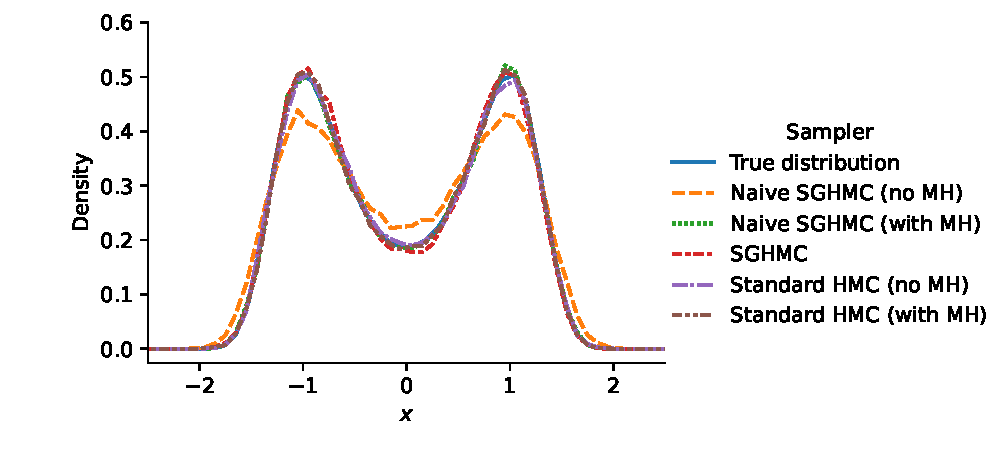
\includegraphics[width=0.9\textwidth]{Figures/synthetic.pdf}
    \caption{Samples from $\log p(x) \propto 2 x^2 - x^ 4$ for different sampling configurations}
    \label{fig:synthetic}
\end{figure}
These result seem to verify our that our implementation is correct.
We also see that the sample distributions from both the standard HMC sampler and the SGHMC sampler closely resembles the true distribution. 
The naive SGHMC sampler does seems to break down when no MH step is included, and since we also compare with regular HMC with no MH step, this demonstrates that it may not be purely down to omitting the MH step. 

If we include an MH step, the naive approach also seem to work, however we are not adding any noise to $E(\cdot)$ when performing the MH step, corresponding to calculating $E(\cdot)$ across the whole data set. 
This is impractical in the context of deep learning, but one could imagine an alternative naive HMC approach where an MH step based on each individual batch of data. 

This experiment also doesn't address whether noise the dynamics of \cref{eq:sghmc-model} are even reasonable as a model for the noise introduced through batching the gradient. 

In order to address these points, we perform an additional simulation experiment. 
This is also to demonstrate the relevance of the different methods in the context of MCMC inference.
We consider the polynomial model of $P(x) = -x + \frac{1}{2}x^2 + \frac{1}{3}x^3$, 
and with $\epsilon \sim \mathcal{N}(0, 1)$, consider a set learning points $y_i = P(x_i) + \epsilon$ for $i=1,\dots,15$, where $x_i$ are linearly spaced over the interval $[-3, 3)$ with a small amount of noise added. 
We then consider the problem of bayesian polynomial regression with known noise $\sigma=1$ and the regression model:
\begin{align*}
    P(x) = a_0 + a_1 x+a_2 x^2 + a_3 x^3
\end{align*}
where each parameter are given a $\mathcal{N}(0, 1)$ prior.
The exact parameter posterior $p(a|x,y)$ for this regression problem is known, and can therefore be compared to the sampled distribution of the samplers. 
More specifically, three sampling strategies are considered, regular HMC conditioned on all data points, HMC where each sample is based on a batch of 5 observations, and SGHMC also with batches of 5 observations.
For demonstration, a plot of the sampled joint distribution of $a_1$ and $a_3$ can be seen in \cref{fig:simulated_joint_comp}.
\begin{figure}[htbp]
    \centering
    \begin{subfigure}[b]{0.4\textwidth}
        \centering
        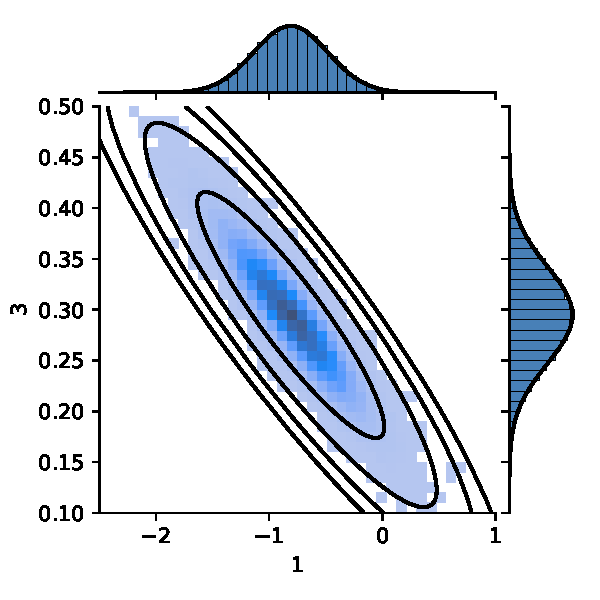
\includegraphics[width=\textwidth]{Figures/simulated_joint_HMC_15.pdf} 
        \caption{HMC conditioned on all data points.}
    \end{subfigure}
    \begin{subfigure}[b]{0.4\textwidth}
        \centering
        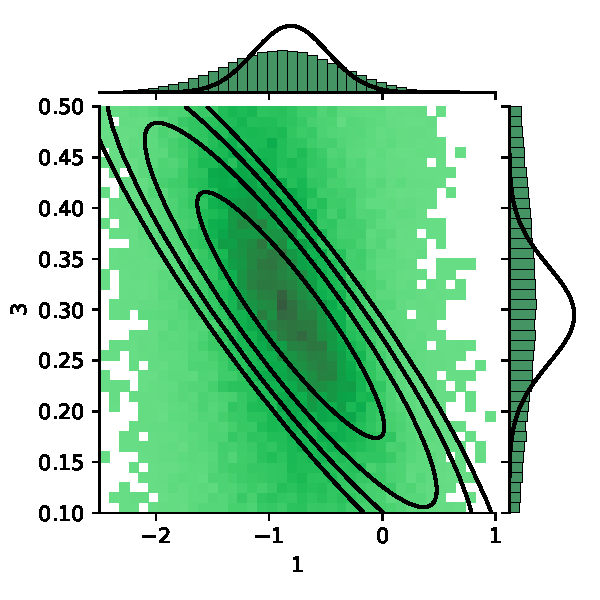
\includegraphics[width=\textwidth]{Figures/simulated_joint_HMC_5.pdf} 
        \caption{HMC with batch size 5}
    \end{subfigure}
    \begin{subfigure}[b]{0.4\textwidth}
        \centering
        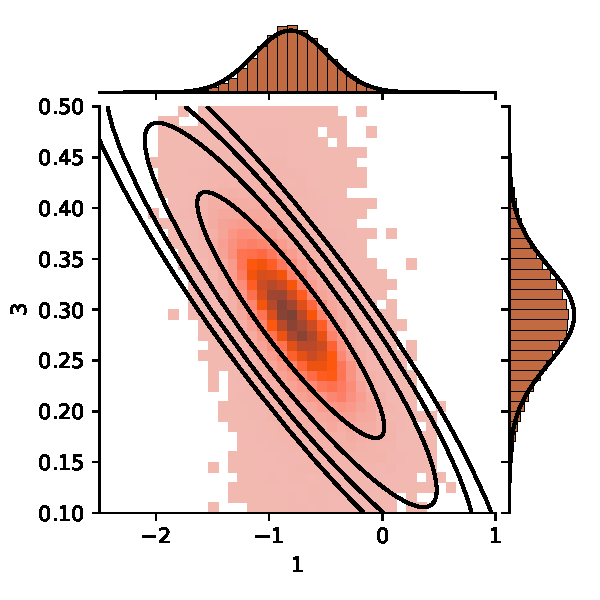
\includegraphics[width=\textwidth]{Figures/simulated_joint_SGHMC_5.pdf} 
        \caption{SGHMC with batch size 5}
    \end{subfigure}
    \caption{Joint distribution of samples for $a_1$ and $a_3$ for the polynomial regression example for HMC and SGHMC for different batch sizes, with the actual posterior density also shown.}
    \label{fig:simulated_joint_comp}
\end{figure}
We find that the also with this approach to the naive SGHMC the batched HMC doesn't, with the sampled posterior having 

with not even the marginal densities being anywhere close to the actual parameter posterior.
Notably, the SGHMC seems to provide a more reasonable estimate, however still with some overdispersion.
In the following section, a possible improvement upon this algorithm is discussed.
